\documentclass[12pt]{article}
\usepackage[version=3]{mhchem} % Package for chemical equation typesetting
\usepackage{siunitx} % Provides the \SI{}{} and \si{} command for typesetting SI units
\usepackage{amsmath} % Required for some math elements 
\usepackage[english]{babel}
\usepackage{natbib}
\usepackage{url}
% * <agoidel2019@mka.org> 2017-03-01T02:11:07.729Z:
%
% ^.
\usepackage[utf8x]{inputenc}
\usepackage[hidelinks]{hyperref} % Clickable references
\usepackage[table,xcdraw]{xcolor}

\usepackage{graphicx}
\graphicspath{{images/}}
\usepackage{parskip}
\usepackage{fancyhdr}
\usepackage{vmargin}
\setmarginsrb{3 cm}{2.5 cm}{3 cm}{2.5 cm}{1 cm}{1.5 cm}{1 cm}{1.5 cm}

\title{Percent Water in a Hydrate}								% Title
\author{Aaron C. Goidel}								% Author
\date{\today}											% Date

\makeatletter
\let\thetitle\@title
\let\theauthor\@author
\let\thedate\@date
\makeatother

\pagestyle{fancy}
\fancyhf{}
\rhead{\theauthor}
\lhead{\thetitle}
\cfoot{\thepage}

\begin{filecontents*}{image.bib}
@ONLINE {Burner,
    author = "Flinn Scientific",
    title  = "Percent Water in a Hydrate",
     note = {Note: [This is not the exact reference, the image was taken from a PDF that was supplied as part of this assignment, it is from the Percent Water in a Hydrate lab packet from Flinn Scientific.]},
    url    = "https://www.flinnsci.com"

}
\end{filecontents*}


\begin{document}

%%%%%%%%%%%%%%%%%%%%%%%%%%%%%%%%%%%%%%%%%%%%%%%%%%%%%%%%%%%%%%%%%%%%%%%%%%%%%%%%%%%%%%%%%

\begin{titlepage}
	\centering
	\vspace*{0.5 cm}
	
\includegraphics[scale = 0.2]{Shield.jpg}\\[1.0 cm]	% School Logo
		\textsc{\LARGE Montclair Kimberley Academy}\\[2.0 cm]	% School Name
		\textsc{\Large Chemistry Honors}\\[0.5 cm]				% Course Code
		\textsc{\large Ms. Thompson}\\[0.5 cm]				% Course Name
		\rule{\linewidth}{0.2 mm} \\[0.4 cm]
		{ \huge \bfseries \thetitle}\\
		\rule{\linewidth}{0.2 mm} \\[1.5 cm]
			
		\begin{minipage}{0.4\textwidth}
			\begin{flushleft} \large
				\emph{Author:}\\
				\theauthor
			\end{flushleft}
		\end{minipage}~
		\begin{minipage}{0.4\textwidth}
			\begin{flushright} \large
				\emph{Lab Partner:} \\
				Andrew Rosamilia 									% Lab partner name 
			\end{flushright}
		\end{minipage}\\[2 cm]
			
		{\large February 13, 2017}\\[2 cm]
		 
		\vfill
			
		\end{titlepage}
		
		%%%%%%%%%%%%%%%%%%%%%%%%%%%%%%%%%%%%%%%%%%%%%%%%%%%%%%%%%%%%%%%%%%%%%%%%%%%%%%%%%%%%%%%%%
		
		\tableofcontents
		\listoftables
		\listoffigures
		\pagebreak
		
		%%%%%%%%%%%%%%%%%%%%%%%%%%%%%%%%%%%%%%%%%%%%%%%%%%%%%%%%%%%%%%%%%%%%%%%%%%%%%%%%%%%%%%%%%
		
		\section{Introduction}
		\subsection{Purpose}
		The purpose of this lab is the analyze the percent of water in a crystalline hydrate and to use the data collected to identify the hydrate from a lost of possible hydrates.
		\subsection{Pre-Lab Questions}
		\begin{enumerate}
			\item Briefly describe three general safety rules for working with a Bunsen burner.
			      \begin{enumerate}
			      	\item Keep loose articles of clothing and long hair at a safe distance from any open flame.
			      	\item Never reach any extremity over top a flame.
			      	\item Use discretion and never leave a burning flame unattended.
			      \end{enumerate}
			\item Using the given data: calculate the mass of the hydrate, the mass of water lost during heating, and the percent water in the hydrate.
			      \begin{enumerate}
			      	\item \(20.75g - 18.42g = 2.33g\)
			      	\item \(20.75g - 20.41g = 0.34g\)
			      	\item \(\frac{0.34g}{20.75g}=0.0164\cdot 100\%=1.64\%\)
			      \end{enumerate}
			\item Fill out table below:
			      \begin{table}[h]
			      	\centering
			      	\caption{Pre-Lab Table (\ce{BaCl2} Hydrates)}
			      	\label{pre-lab}
			      	\begin{tabular}{lllll}
			      		                                       & \cellcolor[HTML]{C0C0C0}\ce{BaCl2} & \cellcolor[HTML]{C0C0C0}\ce{BaCl2*H2O} & \cellcolor[HTML]{C0C0C0}{\color[HTML]{000000} \ce{BaCl2*2H2O}} & \cellcolor[HTML]{C0C0C0}\ce{BaCl2*3H2O} \\
			      		Sum of atomic masses (\ce{BaCl2})      & 208.23                             & 208.23                                 & 208.23                                                         & 208.23                                  \\
			      		Sum of atomic masses (\ce{nH2O})       & 0                                  & 18.02                                  & 36.04                                                          & 54.06                                   \\
			      		Sum of atomic masses (\ce{BaCl2*nH2O}) & 208.23                             & 226.25                                 & 244.27                                                         & 262.29                                  \\
			      		Percent water in hydrate               & 0\%                                & 7.96\%                                 & 14.75\%                                                        & 20.61\%                                 
			      	\end{tabular}
			      \end{table}
			\item What is the most likely formula for Barium Chloride Hydrate?
			      \begin{itemize}
			      	\item[] \ce{BaCl2*2H2O}
			      \end{itemize}
		\end{enumerate}
		
		\newpage
		\section{Procedure}
		\begin{enumerate}
			\item Observe and record initial observations of the crystalline hydrate.
			\item Set up stand and clamp such that a Bunsen burner can be easily moved under the the test tube with some clearance (see Fig. 1).
			      \begin{figure}[h]
			      	\centering
			      	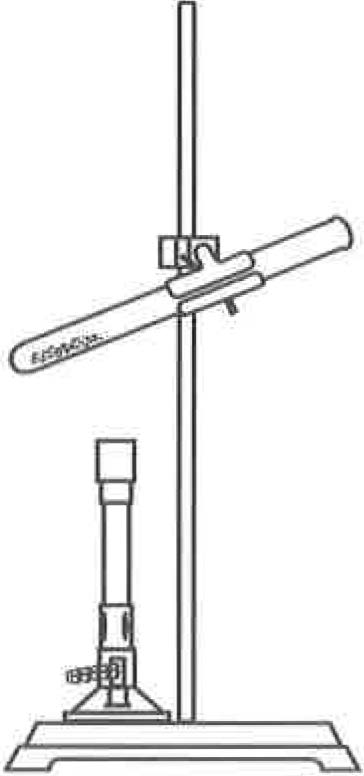
\includegraphics[scale = 0.75]{Tube_Stand}
			      	\hspace*{15pt}\hbox{\scriptsize Credit:\thinspace{\small\itshape Flinn Scientific}}
			      	\caption{Test tube and burner setup}
			      \end{figure}
			\item Measure and record the mass of the test tube for later use.
			\item Using a spatula weigh out 2g of the crystalline hydrate into the test tube.
			\item While using a test tube clamp to hold tube horizontally tap the tube to spread out hydrate (see Fig. 1).
			\item Slide test tube into clamp so that it is almost horizontal and tighten clamp to fix tube into place (see Fig. 1).
			\item Ignite the Bunsen burner and heat bottom of test tube, constantly moving the burner in a sweeping motion (Do this until no more vapor is coming out of the tube).
			\item Allow tube to cool.
			\item Weigh tube with anhydrous salt in it, record results.
			\item Record any physical observations.
		\end{enumerate}
		\newpage
		\section{Data}
		% Please add the following required packages to your document preamble:
		% \usepackage[table,xcdraw]{xcolor}
		% If you use beamer only pass "xcolor=table" option, i.e. \documentclass[xcolor=table]{beamer}
		% Please add the following required packages to your document preamble:
		% \usepackage[table,xcdraw]{xcolor}
		% If you use beamer only pass "xcolor=table" option, i.e. \documentclass[xcolor=table]{beamer}
		\begin{table}[h]
			\centering
			\caption{Mass of Hydrate Before and After Heating (Unknown C)}
			\label{lab-data}
			\begin{tabular}{l|l|l|l|}
				\cline{2-4}
				                                      & \cellcolor[HTML]{C0C0C0}Total Mass & \cellcolor[HTML]{C0C0C0}Mass of Hydrate & \cellcolor[HTML]{C0C0C0}Observations                     \\ \hline
				\multicolumn{1}{|l|}{Empty Test Tube} & 17.06g                             & N/A                                     & \begin{tabular}[c]{@{}l@{}}It's an empty test tube,      \\ not much to report\end{tabular} \\ \hline
				\multicolumn{1}{|l|}{Before Heating}  & 19.00g                             & 1.94g                                   & \begin{tabular}[c]{@{}l@{}}Hydrate is a deep blue color. \\ There are visible crystals.\end{tabular} \\ \hline
				\multicolumn{1}{|l|}{After Heating}   & 18.30g                             & 1.24g                                   & \begin{tabular}[c]{@{}l@{}}The substance has turned to   \\ an ashy white-grey color.\end{tabular} \\ \hline
			\end{tabular}
		\end{table}
		
		\section{Analysis}
        \subsection{Possible Known Hydrates}
        % Please add the following required packages to your document preamble:
% \usepackage[table,xcdraw]{xcolor}
% If you use beamer only pass "xcolor=table" option, i.e. \documentclass[xcolor=table]{beamer}
% Please add the following required packages to your document preamble:
% \usepackage[table,xcdraw]{xcolor}
% If you use beamer only pass "xcolor=table" option, i.e. \documentclass[xcolor=table]{beamer}
% Please add the following required packages to your document preamble:
% \usepackage[table,xcdraw]{xcolor}
% If you use beamer only pass "xcolor=table" option, i.e. \documentclass[xcolor=table]{beamer}
% Please add the following required packages to your document preamble:
% \usepackage[table,xcdraw]{xcolor}
% If you use beamer only pass "xcolor=table" option, i.e. \documentclass[xcolor=table]{beamer}
% Please add the following required packages to your document preamble:
% \usepackage[table,xcdraw]{xcolor}
% If you use beamer only pass "xcolor=table" option, i.e. \documentclass[xcolor=table]{beamer}
\begin{table}[h]
\centering
\caption{Atomic Masses and Percent Water in the Hydrates}
\label{results}
\begin{tabular}{l|l|l|l|}
\cline{2-4}
                                                                                                      & \cellcolor[HTML]{C0C0C0}\ce{CuSO4*5H2O}                                     & \cellcolor[HTML]{C0C0C0}\ce{MnCl2*4H2O}                                        & \cellcolor[HTML]{C0C0C0}\ce{ZnSO4*7H2O}                             \\ \hline
\multicolumn{1}{|l|}{\begin{tabular}[c]{@{}l@{}}Sum of atomic masses\\ (anhydrous salt)\end{tabular}} & 159.61g/mol                                                                 & 125.84g/mol                                                                     & 161.47g/mol                                                         \\ \hline
\multicolumn{1}{|l|}{\begin{tabular}[c]{@{}l@{}}Sum of\\ atomic masses (\ce{nH2O})\end{tabular}}        & 90.10g/mol                                                                  & 72.08g/mol                                                                     & 126.14g/mol                                                         \\ \hline
\multicolumn{1}{|l|}{\begin{tabular}[c]{@{}l@{}}Sum of atomic masses\\ (salt\ce{*nH2O})\end{tabular}} & 249.71g/mol                                                                 & 197.92/mol                                                                    & 287.61g/mol                                                         \\ \hline
\multicolumn{1}{|l|}{Percent water in hydrate}                                                        & 36.08\%                                                                     & 36.41
\%                                                                        & 43.86\%                                                             \\ \hline
\multicolumn{1}{|l|}{Name of hydrate}                                                                 & \begin{tabular}[c]{@{}l@{}}Copper (II) Sulfate \\ Pentahydrate\end{tabular} & \begin{tabular}[c]{@{}l@{}}Manganese (II) Chloride\\ Tetrahydrate\end{tabular} & \begin{tabular}[c]{@{}l@{}}Zinc Sulfate\\ Heptahydrate\end{tabular} \\ \hline
\end{tabular}
\end{table}

\newpage
\subsection{Results}
\subsubsection{Result Calculations}
Hydrate: Unknown C\\
Mass of Test Tube: 17.06g
\\\\
Original Mass of Hydrate: 
\[19.00g - 17.06g = 1.94g\]

Mass of Water Lost Upon Heating:
\[19.00g - 18.30g = 0.70g\]
Percent Water in Hydrate:
\[\frac{0.70g}{1.94g}=.36\cdot 100\% = 36\%\]

\subsubsection{Identification of Hydrate}
The identity of the unknown substance (Unknown C) is Copper(II) Sulfate Pentahydrate. The data shows that the percent of water contained in the unknown substance was roughly 36\% which, of the possible compounds, was closest to the theoretical percent of water in Copper(II) Sulfate Pentahydrate, which was 36.08\%. In addition to this the color of the hydrate was blue prior to heating and compounds containing copper are blue/green in color.

\subsubsection{Percent Error}
\[\mbox{Percent Error}=100\%\left|\frac{\mbox{experimental}-\mbox{expected}}{\mbox{expected}}\right|\]
\[100\%\left | \frac{36-36.08}{36.08} \right |=100\%\left | \frac{-0.08}{36.08} \right |=100\%\left | -.0022 \right |=0.22\%\]

\newpage
\subsection{Discussion}
\subsubsection{Question 5}
Precision is very important in experimental science. Precision refers to the consistency of a measurement or procedure in producing results. Any good experiment must be repeatable, thus precise. Precision also refers to how detailed a measurement is, the degree of precision in an experiment is very important in finding correlations in data. The results in this experiment were rather precise. All of the measurements were taken with a high and consistent degree of precision, leading to only a 0.22\% margin of error.

\subsubsection{Question 6}
The unknown hydrate is a homogeneous mixture. The reason it is not a pure substance is there are two chemicals involved in making a hydrate, a salt (in this case \ce{CuSO4}) and water.

\subsubsection{Question 7}
The conversion of the hydrate to its anhydrous salt is a physical change. This is because in heating the hydrate all that is happening is the water evaporates out and state changes are not chemical changes. No new substances are being made.

\subsubsection{Question 8}
If the water was not completely evaporated from the hydrate the calculations could have been corrupted, this is because the experimental mass of the water in the hydrate is based off of the change in mass between the hydrate before and after heating. If all of the water is not evaporated the hydrate will be more massive afterwards leading to less water being calculated to exist in the hydrate. This would lead to an underestimated percent of water in the hydrate.

\subsubsection{Question 9}
Had some of the anhydrous salt decomposed and been released as a gas during the heating process the final mass would have been less than it should have been, leading to the calculated mass of water to be higher, thus increasing the final experimental result.

\subsubsection{Question 10}
The chemist should use the first measurement for the mass of the crucible, cover, and dehydrated sample. This is because she only measured the mass of the crucible and cover once and that was before the first trial. The data shows that the final mass decreases slightly each time the experiment is done which could mean the mass of the crucible is changing and the most accurate measurement would be the one taken before the crucible could start to lose mass. 
		\newpage
        \nocite{Burner}
		\bibliographystyle{plainnat}
        \bibliography{image}
		
		
\end{document}